
\usetikzlibrary{positioning}

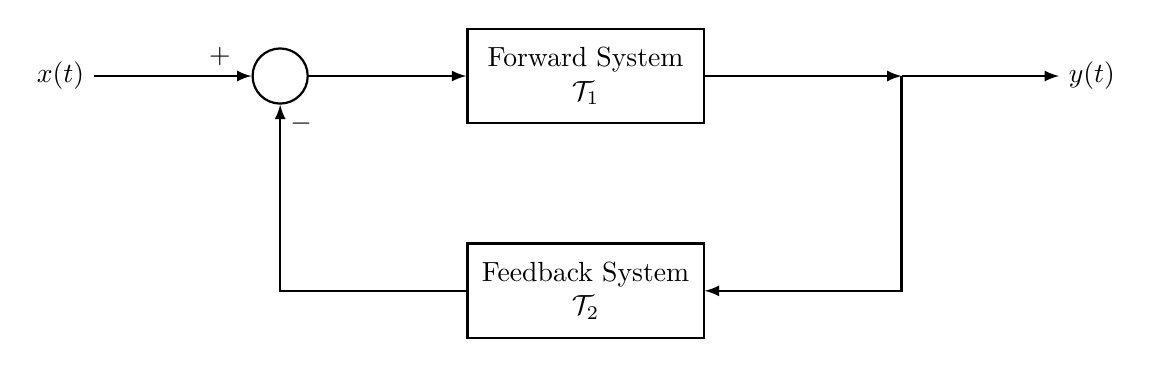
\begin{tikzpicture}[
	% Set the default distance between nodes.
	node distance=1.5cm and 2cm
	]
	% Define custom styles to make the code cleaner and more reusable.
	\tikzset{
		block/.style={draw, rectangle, minimum height=1.2cm, minimum width=3cm, align=center, thick},
		sum/.style={draw, circle, inner sep=0pt, minimum size=7mm, thick},
		line/.style={-latex, thick} % Use -latex for a nicer arrowhead
	}
	
	% === NODES ===
	% Place the nodes for the diagram.
	
	\node (input) {\(x(t)\)};
	\node[sum, right=of input] (summer) {};
	\node[block, right=of summer] (sys1) {Forward System \\ \(\mathcal{T}_1\)};
	\node[coordinate, right=2.5cm of sys1] (split) {};
	\node[right=of split] (output) {\(y(t)\)};
	\node[block, below=of sys1] (sys2) {Feedback System \\ \(\mathcal{T}_2\)};
	
	% === CONNECTIONS ===
	% Draw the lines and arrows connecting the nodes.
	
	\draw[line] (input) -- node[pos=0.8, above] {\(+\)} (summer);
	\draw[line] (summer) -- (sys1);
	\draw[line] (sys1) -- (split);
	\draw[line] (split) -- (output);
	
	% Feedback Path
	\draw[line] (split) |- (sys2);
	\draw[line] (sys2) -| node[pos=0.95, right] {\(-\)} (summer);
\end{tikzpicture}